\section{Проектирование и реализация} % (fold)
\label{sec:arch_and_realization}


Разработанное программное обеспечение представляет из себя приложение, написанное на фреймворке \ror.
Приложение предназначено для получения новинок музыкальной индустрии или, другими словами, музыкальных релизов выбранных пользователем музыкантов.

\subsection{Проектирование приложения}
\label{sub:arch_and_mod:design}
При проектировании приложения обязательно следует учитывать фактор изменяемости и заложить возможности расширяемости. Учитывая эти факторы, можно приступать к написанию приложения с осознанием того факта, что в будущем не придется переписывать его полностью с нуля. Все, что будет нужно -- это добавить новые компоненты, то есть расширить систему.

В случае сервиса, предоставляющего возможность получения новинок музыкальной индустрии, расшираяемость будет выражаться в том, чтобы была возможность добавить новые сторонние сервисы, которые предоставляют свой API для использования ресурсов.

Проектирование БД в данной работе можно начать с модели пользователя. Пользователь -- одна из ключевых фигур в работе сервиса. Пользователю должны быть доступны:

\begin{itemize}
  \item регистрация;
  \item аутентификация;
  \item авторизация;
  \item доступ к непосредственным возможностям сервиса.
\end{itemize}

Для упрощения реализации вышеуказанных возможностей в сервисе используется библиотека Devise. Она диктует создание модели пользователя определенным образом, чтобы можно было легко использовать встроенные в нее инструменты: регистрация, аутентификация, восстановление пароля, подтверждение регистрации и др. Таким образом, модель пользователя будет состоять из следующих полей:

\begin{itemize}
  \item id;
  \item email;
  \item encrypted\_password;
  \item reset\_password\_token;
  \item confirmation\_token;
  \item created\_at;
  \item updated\_at.
\end{itemize}

В действительной таблице пользователя полей несколько больше, но этого объема достаточно, чтобы передать основные направления проектирования модели пользователя.

Далее рассмотрим модель артиста. Учитывая тот факт, что в сервисе будут использоваться сторонние приложения и их API, нужно отметить, что у каждого из них свое строение. В данной версии сервиса будет использоваться три сторонних приложения, информация двух из которых будет по мере использования сервиса сохраняться в БД. Эти два сервиса: Discogs\footnote{\url{https://discogs.com/}} и Rate Your Music\footnote{\url{https://rateyourmusic.com/}}. В каждом из этих сервисов есть информация об артистах. Поэтому было принято решение создать две модели: DiscogsArtistsInfo (модель, которая отвечает за сохранение информации из веб-приложения Discogs) и RymArtistsInfo (отвечает за сохранение информации из веб-приложения, которое называется Rate Your Music).

Модель DiscogsArtistsInfo, учитывая структуру информации в приложении Discogs, включает в себя следующие поля:

\begin{itemize}
  \item id;
  \item image\_url;
  \item created\_at;
  \item updated\_at.
\end{itemize}

Учитывая структуру информации в приложении Rate Your Music, модель RymArtistsInfo включает в себя следующие поля:

\begin{itemize}
  \item id;
  \item formed\_year;
  \item disbanded\_year;
  \item genres;
  \item created\_at;
  \item updated\_at.
\end{itemize}

Также в сервисе присутствует модель, которая выступает как модель артиста уже внутри системы. Она будет соединяться с вышеописанными моделями артиста через промежуточную модель, которая будет описана позже. Таким образом, модель ArtistIdentity включает в себя следующие поля:

\begin{itemize}
  \item id;
  \item name;
  \item created\_at;
  \item updated\_at.
\end{itemize}

Музыкальная публикация, или релиз, также является ключевым понятием в сервисе. Так как работа происходит с двумя сторонними приложениями, для хранения информации о музыкальных публикациях происходит через две модели: DiscogsReleasesInfo (отвечает за сохранение информации из сервиса Discogs) и RymReleasesInfo (отвечает за сохранение информации из сервиса Rate Your Music).

DiscogsReleasesInfo содержит следующие поля:

\begin{itemize}
  \item id;
  \item format\_type;
  \item track\_list;
  \item genres;
  \item label;
  \item style;
  \item created\_at;
  \item updated\_at.
\end{itemize}

RymReleasesInfo содержит следующие поля:

\begin{itemize}
  \item id;
  \item format\_type;
  \item track\_list;
  \item genres;
  \item descriptors;
  \item created\_at;
  \item updated\_at.
\end{itemize}

Поле, обозначаемое как format\_type, несет в себя информацию о типе релиза: сингл, extended\_play и др. Поле descriptors содержит в себе дополнительную информацию, которая может говорить об релизе и по которой потом можно проще производить поиск.

Однако так же, как и с организацией хранения артистов, необходимо иметь модель музыкальной публикации внутри системы. Такой моделью является ReleaseIdentity и включает в себя следующие поля:

\begin{itemize}
  \item id;
  \item year\_released;
  \item format\_type;
  \item created\_at;
  \item updated\_at.
\end{itemize}

Чтобы система была расширяема, необходимо сделать возможность добавления различных компонентов. В сервисе, предоставляющем возможность получения новинок музыкальной индустрии, такими компонентами являются сторонние сервисы, предоставляющие доступ к своему API. В данной реализации, как уже было сказано, используются два таких сервиса: Discogs и Rate Your Music. Для обоих сервисов в системе созданы модели как артистов, так и музыкальных публикаций (релизов). Также созданы представления артистов и релизов в самой системе в виде моделей. Для пользователя нет нужды, и даже может быть затруднительно, представлять артистов и релизы в контексте различных сторонних сервисов. Для пользователя удобнее видеть не две или более различных музыкальных публикаций, которые на самом деле являются одной и той же, но и разных сервисов, а видеть одну публикацию, информация о которой расширена и дополнена данными из сторонних API. Таким образом удается не просто избегать дублирования, но и обогащать данные. Со временем можно добавить и больше различных сторонних сервисов. Таким образом, в системе присутствует модель ArtistIdentity, которая дополняется моделями DiscogsArtistsInfo и RymArtistsInfo. Также для обозначения релизов в системе присутствует модель ReleaseIdentity, которая дополняется моделями DiscogsReleaseInfo и RymReleaseInfo. Чтобы связать эти модели, необходимо создать модель Identity, которая будет ссылаться на объекты вышеописанных моделей и включать следующие поля:

\begin{itemize}
  \item id;
  \item entity\_id;
  \item service\_entity\_id;
  \item info\_id;
  \item service\_type;
  \item entity\_type;
  \item created\_at;
  \item updated\_at.
\end{itemize}

Данная модель является надстройкой над вышеописанными моделями и связывает их определенным образом. Поле service\_type содержит имя сервиса, информацию которого содержит. В данной реализации этими именами могут быть "rym" и "discogs". В качестве значений поля entity\_type могут выступать "artist" и "release". На основе entity\_type и service\_type можно info\_id будет ссылаться на нужный объект информации релиза или артиста из того или иного сервиса.

Таким образом, опираясь на вышеописанную структуру данных в сервисе, можно строить приложение, наполняя его бизнес-логикой.

Существует множество подходов для построения архитектуры приложений. В данном дипломном проекте была выбрана трехуровневая архитектура.

\subsection{Трехуровневая архитекутра приложения}
\label{sub:arch_and_mod:mvc}

Архитектура приложения -- это определенный подход в определении взаимоотношений компонентов приложения. Обычно архитектура приложений соответствует задачам разработки. В данном дипломном проекте выбрана трехуровневая архитектура. Эти уровни называются: уровень модели, уровень контроллера и уровень представления. Иначе говоря, MVC~\cite{mvc_doc} -- Model, View, Controller.

Данная архитектура используется во множестве веб-фреймворков. Она удобна тем, что позволяет разделить зоны ответственности между компонентами, облегчить тестирование, придать гибкость разработке. Фреймворк \ror{} и \ajs{} также в своей основе используют данную архитектуру.

\begin{figure}[ht]
\centering
  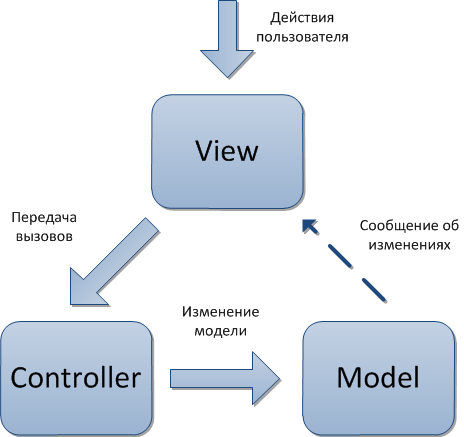
\includegraphics[scale=0.4]{mvc_picture.png}
  \caption{ Схема трехуровневой архитектуры }
  \label{fig:arch_and_mod:mvc:picture}
\end{figure}

\subsubsection{Уровень модели}
\label{sub:arch_and_mod:mvc:model}
~\newline
\indent Уровень модели -- один из трех уровней в MVC-архитектуре. Его обязанности можно разделить на две категории:

\begin{itemize}
  \item бизнес-логика приложения;
  \item управление связью в базой данных.
\end{itemize}

Бизнес-логика включает в себя определенные правила, отношения и принципы, которые должны существовать в приложении. Эти правила могут быть выражены как в коде самого приложения, так и базе данных. Однако в данном дипломном проекте бизнес-логика содержится именно в коде приложения, а именно в ruby-классах, наследующихся от класса ActiveRecord::Base, который является стандартом де-факто для моделей, использующихся во фреймворке \ror{}.

В данном дипломном проекте присутствует класс ReleaseIdentity, который используется для хранения и обработки объектов музыкальных публикаций. Пример реализации класса ReleaseIdentity представлен на листинге~\ref{lst:arch_and_mod:mvc:model:release_identity_class_definition}:
\begin{lstlisting}[style=fsharpstyle,caption={Базовая реализация класса ReleaseIdentity}, label=lst:arch_and_mod:mvc:model:release_identity_class_definition]
class ReleaseIdentity < ActiveRecord::Base
end
\end{lstlisting}

Классы-наследники класса ActiveRecord::Base обладают богатым функционалом. Они содержат в себе возможности валидирования, организации связей между объектами, возможностями создания транзакций, сложных запросов в БД и многими другими. Подробнее об этом будет написано несколько позже, когда будет рассматриваться взаимодействие с БД.

Ярким примером бизнес-логики может служить проверка корректности конструируемых объектов. Например, название артиста не должно быть пустым и содержать только текстовые данные. Или же год начала карьеры артиста не может быть отрицательными или больше нынешнего года по значению. Все это реализуется в \ror{} с помощью механизма валидации.

В данном дипломном проекте присутствует класс RymArtistsInfo, который используется для хранения результатов работы с сервисом Rate Your Music. В этом классе присутствуют следующие поля:

\begin{itemize}
  \item id -- уникальный идентификатор записи в таблице;
  \item formed\_year -- год формирования музыкальной группы(исполнителя);
  \item disbanded\_yead -- год окончания деятельности музыкальной группы (исполнителя);
  \item genres -- жанры, которые присущи музыкальной группе(исполнителю);
  \item created\_at -- дата создания записи в БД приложения;
  \item updated\_at -- дата обновления записи в БД приложения.
\end{itemize}

В данном случае годы формирования и окончания деятельности музыкальной группы исполнителя должны придерживаться правил, описанных выше. Также строка, содержащая жанры, не может иметь длину, менее 2 символов. Для обеспечения этой части бизнес-логики я воспользовался инструментарием фреймворка \ror{}. Используя метод validates, можно добиться проверки определенных правил перед сохранением записи, чтобы хранить в базе только корректные записи. Также существует метод validate, в который передается название метода, в котором можно описать более сложную логику. Таким образом можно проверить то, что год окончания деятельности музыкальной группы больше или равен году начала карьеры. Пример использования продемонтрирован на листинге ~\ref{lst:arch_and_mod:mvc:model:rym_artists_info_validations}:

\begin{lstlisting}[style=fsharpstyle,caption={Реализация валидации в классе RymArtistsInfo}, label=lst:arch_and_mod:mvc:model:rym_artists_info_validations]
class RymArtistsInfo < ActiveRecord::Base
  validates :formed_year
  validates :disbanded_year, numericality: {only_integer: true, greated_than: 0, less_than: DateTime.now.year}
  validates :genres, length: {minimum: 2}
  validate disbanded_more_or_eql_formed

  private

  def disbanded_more_or_equal_formed
    disbanded_year >= formed_year
  end
end
\end{lstlisting}

Фреймворк \ror{} предлагает еще один полезный инструмент, который называется "функция обратного вызова". Такие функции существуют и на уровне базы данных, но в этом и состоит преимущество веб-фреймворка - позволять более компактно и удобно писать необходимый функционал. Функции обратного вызова работают таким образом, что в определенные моменты жизненного цикла объектов, такие, как перед сохранением, удалением или валидированием объекта, вызываются методы, в который можный поместить необходимый для этого момента код. Это еще одно преимущество слоя модели, потому как позволяет избегать длинных цепочек вызовов методов, а воспользоваться удобным интерфейсом для обработки моментов жизненного цикла. В \ror{} такие моменты обрабатываются путем добавления методов:
\begin{itemize}
  \item before\_save;
  \item before\_create;
  \item before\_validate;
  \item around\_save;
  \item after\_save;
  \item after\_update.
\end{itemize}

Пример функции обратного вызова представлен на листинге~\ref{lst:arch_and_mod:mvc:model:callback}:

\begin{lstlisting}[style=fsharpstyle,caption={Пример получения артистов по определенным параметрам}, label=lst:arch_and_mod:mvc:model:callback]
  class RymReleasesInfo < ActiveRecord::Base
    after_save :set_link_to_identity

    private

    def set_link_to_identity
      ReleaseIdentity.find_or_create_by(
        title: title,
        artist: artist
      )
    end
  end
\end{lstlisting}

Стоит обратить внимание на тот факт, что с ростом приложений модели включают в себя все больше логики и становятся очень большими. Минус этого состоит в том, что происходит нарушение одного из принципов объектно-ориентированного программирования. Это принцип единственной ответственности класса. Он нарушается в тот момент, когда класс выполняет много различных функций: используется для подключения к БД, содержания бизнес-логики, создания других объектов и т.д. Однако существует способ улучшения данной архитектуры путем введения в слой модели дополнительного компонента - сервиса. Сервисы - это такие классы или модули, который содержат в себе код, который можно извлечь из модели, чтобы ее не перегружать. Например, сервисы могут содержать в себе код обращения в стороннему приложению, либо расчет цен и многое другое. Более того, код сервисов может использоваться в различных местах, тем самым обеспечивая модульность. Это помогает проще тестировать. Кроме этого, сервисы реализуют принцип инкапсуляции, то есть принцип сокрытия реализации. Имеется в виду, что коду, использующему сервис, необязательно знать, как именно реализован тот или иной метод. Если сервис отвечает за работу с поиском и передачей музыкальных публикаций, то коду, работающему с этим сервисом не важно, берет сервис публикации с помощью API, делает запрос в БД или же эти публикации просто лежат в массиве в памяти приложения. Сам фреймворк не предполагает наличие сервисов, но никак не препятствует их созданию. Пример сервиса, выполняющего функцию доступа к одному из сторонних приложений ~\ref{lst:arch_and_mod:mvc:model:discogs_service_example}:

\begin{lstlisting}[style=fsharpstyle,caption={Пример получения артистов по определенным параметрам}, label=lst:arch_and_mod:mvc:model:discogs_service_example]
  module DiscogsDataService

    def self.find_artists_by_name(name)
      DiscogsApiWrapper.find_artists(name: name)
    end

    def self.find_release_by_title(title)
      DiscogsApiWrapper.find_release(title: title)
    end

  end
\end{lstlisting}

Также слой модели ответственнен за работу с базой данных. Большим преимуществом данного слоя вообще и конкретно в реализации библиотеки ActiveRecord является то, что данная ORM имеет один интерфейс для работы с различными базами данных, будь то PostgreSQL, MySQL, SQLite или другие. Используя классы, которые унаследованы от класса ActiveRecord::Base, можно обращаться к базе данных для того, чтобы получить список артистов, релизов или пользователей с помощью языка Ruby. Например, если необходимо сделать выборку артистов, год начала деятельности которых больше какого-то определенного, при этом не выбирая все поля, а только год прекращения деятельности и дату создания записи в БД, используется код, указанный в листинге ~\ref{lst:arch_and_mod:mvc:model:select_artist_where_year}:

\begin{lstlisting}[style=fsharpstyle,caption={Пример получения артистов по определенным параметрам}, label=lst:arch_and_mod:mvc:model:select_artist_where_year]
  artists = RymArtistsInfo.select(:disbanded_year, :created_at).where('formed_year > ?', Date.new(2000, 4, 3))
\end{lstlisting}

Таким образом, классы, унаследованные от ActiveRecord::Base предоставляют удобный интерфейс, который помогает не писать чистый SQL-код. Возможности ActiveRecord::Base не ограничиваются простыми запросами. Существуют методы, которые позволяют делать сложные запросы, избегать проблемы "N+1" и т.д.

Стоит упомянуть, что веб-фреймворк AngularJS также использует слой модели. В качестве объектов модели в AngularJS используются так называемые ресурсы. Ресурсы используются преимущественно для работы с запросами к API. Ресурсы в AngularJS предоставляют возможность использования как стандартных REST-запросов, так и создания пользовательских. Пример ресурса на AngularJS приведен в листинге ~\ref{lst:arch_and_mod:mvc:model:angular_artists_resource}:

\begin{lstlisting}[style=fsharpstyle,caption={Пример получения артистов по определенным параметрам}, label=lst:arch_and_mod:mvc:model:angular_artists_resource]
  app = angular.module('app')

  app.factory 'Artist', ['\$resource', (\$resource) ->
    \$resource('/artists/:id', { id: '@_id' }, {
      short_info: {method: 'GET', url: '/artist/:id/short_info'}
      extended_info: {method: 'GET', url: '/artists/:id/extended_info'}
      last_releases: {method: 'GET', url: '/artists/:id/last_releases'}
    })
  ]
\end{lstlisting}

\subsubsection{Уровень контроллера}
\label{sub:arch_and_mod:mvc:controller}
~\newline
\indent Уровень контроллера -- это второй уровень в MVC-архитектуре, отвечающий за соединение слоя модели и слоя представления. В контроллерах принятно получать информацию через модели из базы данных и отображать некоторым образом эту информацию в представлениях. Представления могут быть как динамическими HTML-страницами, так и просто JSON-информацией.

Контроллеры присутствуют, как в \ror{}, так и в AngularJS. Контроллеры в \ror{} принимают запросы и возвращают ответ. Контроллеры в AngularJS ответственны за то, чтобы инициализировать некоторую информацию, отображать ее в представлениях и потом следить за обновлениями, происходящими на странице. Рассмотрим реализации котроллеров более подробно.

Фреймворк \ror{} заточен под REST. Таким образом, при написании контроллеров приветствуется написание методов этих контроллеров в ресурсном стиле. В системе есть ресурс Artist, то есть модель артиста. Чтобы обрабатывать эту модель в ресурсном виде, необходимо создать реализацию следующих действий:

\begin{itemize}
  \item new - метод для создания нового артиста. Данный метод контроллера может возвращать либо HTML-страницу с формой и некоторыми инициализированными значениями для выбора опций, либо, если контроллер выступает в роли API, просто возвращать некоторые начальные данные для инициализации полей для выбора;
  \item create - метод, в который приходит информация из формы и который должен ее обработать и создать артиста. Если при создании артиста присутствует некоторая логика, желательно вынести ее в отдельный метод модели или же сервис, чтобы не нагружать контроллер лишней ответственностью;
  \item show - метод, который либо возвращает страницу с заполненной информацией об артисте, либо, если контроллер выступает в роли API, возвращать саму информацию об артисте в формате JSON;
  \item edit - метод, который выполняет похожие на метод "new" функции за тем исключением, что предназначен для редактирования, и поля или информация, возвращаемая из метода, уже содержит в себе данные созданного артиста;
  \item update - метод, который берет на себя обязанности по обновлению артиста. По своей функциональности похож на метод "create", но не создает, а обновляет артиста при необходимости;
  \item destroy - метод, который удаляет артиста;
  \item index - метод, в обязанности которого входит работа со списком артистов. Возвращает HTML-страницу с заполненным списком артистов или же возвращает список артистов в JSON-формате.
\end{itemize}

Также контроллер принимает определенные параметры как часть запроса. Например, немаловажной является функциональность пагинации, то есть разделения списка артистов по страницам. Для реализации этой функциональности используется библиотека Kaminari, которая предоставляет простой интерфейс, доступный в контроллерах и HTML-код, который можно использовать в представлениях для отображения элементов управления, содержащих номера страниц и кнопок, которые способны, например, перейти на страницу вперед иди назад, а также на первую или последнюю страницу.

Стоит упомянуть, что контроллер отвечает за то, чтобы параметры, которые приходят в метод обработки ресурса, содержали только необходимые ключи. Это необходимо для того, чтобы обезопасить себя от многих атак. Для выборки параметров существует такой инструмент, как "parameters whitelist", то есть "белый лист параметров". В контроллере описывается private-метод, который указывает, какие параметры допустимы. Название этого метода обычно состоит из двух частей, первая из которых называется именем ресурса, а вторая содержит слово "params". Таким образом, в контроллере артистов этот метод будет называться "artists\_params".

Пример кода контроллера, который обрабатывает ресурс артиста представлен на листинге ~\ref{lst:arch_and_mod:mvc:controller:artists_controller_example}.

\begin{lstlisting}[style=fsharpstyle,caption={Пример получения артистов по определенным параметрам}, label=lst:arch_and_mod:mvc:controller:artists_controller_example]
  class ArtistsController < ApplicationController

    before_action :authenticate_user!

    def index
      authorize! :index, Artist
      @artists = Artist.all
                       .page(params[:page])
                       .per(params[:per])
       respond_to do |format|
        format.js
        format.html
       end
    end

    def new
      authorize! :new, Artist
      @artist = Artist.new
      respond_to do |format|
       format.js
       format.html
      end
    end

    def create
      authorize! :create, Artist
      @artist = Artist.create(artists_params)
      respond_to do |format|
        if @artist.save
          format.html { redirect_to @artist }
          format.json { render :show, status: :created}
        else
          format.html { render :new }
          format.json { render json: @artist.errors, status: :unprocessable_entity }
        end
      end
    end

    def show
      authorize! :show, Artist
      @artist = Artist.find(params[:id])
      respond_to do |format|
       format.js
       format.html
      end
    end

    def edit
      authorize! :show, Artist
      @artist = Artist.find(params[:id])
      respond_to do |format|
       format.js
       format.html
      end
    end

    def update
      authorize! :update, Artist
      @artist = Artist.find(params[:id])
      respond_to do |format|
        if @artist.save
          format.html { redirect_to @artist }
          format.json { render :show, status: :created}
        else
          format.html { render :edit }
          format.json { render json: @artist.errors, status: :unprocessable_entity }
        end
      end
    end

    def destroy
      authorize! :destroy, Artist
      @artist = Artist.find(params[:id])
      redirect_to artists_path
    end

    private

    def artists_params
      params.require(:artist).permit(:name,
                                     :formed_year,
                                     :disbanded_year,
                                     genres: [] )
    end

  end
\end{lstlisting}

Помимо непосредственных обработки запросов и возвращения ответов в обязанности контроллера входит проверять права доступа для определенных методов. Например, список артистов может просматривать и не аутентифицированный пользователь, но создать артиста может только зарегистрированный и аутентифицированный. А изменять пользователя может только пользователь с ролью администратора. В данном случае используется авторизация. То есть в некоторых случаях таких, как, например, редактирование модели артиста, для операции необходим функционал аутентификации и авторизации.

Для реализации авторизации приложения применяется библиотека, которая называется CanCanCan. Принцип работы состоит в том, что разработчики описывают так называемые политики, которые потом используются для проверки прав доступа. Пример написания политик приведен на листинге ~\ref{lst:arch_and_mod:mvc:controller:cancancan_example}.

\begin{lstlisting}[style=fsharpstyle,caption={Пример получения артистов по определенным параметрам}, label=lst:arch_and_mod:mvc:controller:cancancan_example]
  class Ability
    include CanCan::Ability

    def initialize(user)
      role == user.role
      artists_abilities(user, role)
    end

    private

    def artists_abilities(user, role)
      if role == :system_admin
        can [:index, :new, :create, :edit, :update, :show, :destroy]
      else
        can [:index, :new, :create, :show]
      end
    end

  end

\end{lstlisting}

В AngularJS контроллеры выступают в роли связующего звена между представлением и некоторой логикой. В AngularJS присутствует переменная \$scope, которой динамически присваиваются свойства и потом к ним можно получить доступ в представлениях. Так и устроен механизм. В AngularJS есть еще одна возможность, которая позволяет автоматически отслеживать изменения некоторых полей и производить некоторые действия на основе этих изменения. Такая функция называется \$watch, она доступна в контроллерах AngularJS и принимает функцию, аргументами которой являются старое и новое значения отслеживаемого свойства \$scope-переменной. Когда переменная меняется, например, в нашем случае, в строке поиска артиста по имени, мы вводим букву, и, соответственно свойство, примененное к этому полю, меняется, то вызывается функция, переданная в \$watch. Тем временем массив предполагаемых артистов, который при инициализации контроллера является пустым, наполняется артистами, пришедшими с API по запросу, содержащему введенную в поле строку. Код контроллера поиска артиста представлен на листинге ~\ref{lst:arch_and_mod:mvc:controller:angular_controller_example}:

\begin{lstlisting}[language=JavaScript,caption={Пример получения артистов по определенным параметрам}, label=lst:arch_and_mod:mvc:controller:angular_controller_example]
  app = angular.module('app')

  app.controller 'ArtistsSearchController', ['$scope', 'Artist', ($scope, Artist) ->

  $scope.artistTitle = ''
  $scope.artists = []

  $scope.$watch('addedProductId', (newValue, oldValue) ->
    if newValue.length > 2
      Artist.search({title: newValue}, (response) ->
        $scope.artists = response.artists
      )
  )
\end{lstlisting}

\subsubsection{Уровень представления}
\label{sub:arch_and_mod:mvc:view}
~\newline
\indent Уровень представления - это третий слой MVC-архитектуры. Он отвечает отображение информации пользователю. Задача уровня представления - быть понятной и привлекательной. В данном дипломном проекте уровень представления реализуется тремя библиотками: \ror{}(когда используются HTML-страницы в ответах на запросы), AngularJS(когда используются HTML-шаблоны со вставками angular-кода, управляемыми angular-контроллерами) и Bootstrap(когда необходимы стили для элементов и сетка для их размещения).

%% пример кода Ruby on Rails + Bootstrap (artists list)

Фреймворк \ror{} обладает встроенным HTML-препроцессором и позволяет помещать в HTML части ruby-кода. Оно работает таким образом, что в контроллере инициализируются некоторые переменные и потом используются в представлениях. Пример представления, содержащего список артистов, представлен на листинге ~\ref{lst:arch_and_mod:mvc:controller:rails_view_example}:

\begin{lstlisting}[language=HTML5,caption={Пример получения артистов по определенным параметрам}, label=lst:arch_and_mod:mvc:controller:rails_view_example]
  <div class="container">
    <div class="row">
      <div class="col-md-12">
        <%= @artists.each do |artist|%>
          <h2>Title</h2>
          <h3> <%= artist.title %> </h3>
          <div class="image-container">
            <%= artist.main_image_path %>
          </div>
          <%= link_to 'Show details', artists_path(artist), class: 'btn btn-info' %>
        <% end %>
      </div>
    </div>
  </div>
\end{lstlisting}
%% пример кода AngularJS + Bootstrap (search artist)

Аналогичным образом работает и AngularJS с тем отличием, что данные, которыми он пользуется в представлениях, инициализируются в контроллерах. То, как данные попадают в контроллер, уже не заботит представление. В контроллерах AngularJS присутствует переменная \$scope, которая, как клей, связывает контроллер и представление. Пример представления для поиска артиста представлен на листинге ~\ref{lst:arch_and_mod:mvc:controller:angular_view_example}:

\begin{lstlisting}[language=HTML5,caption={Пример получения артистов по определенным параметрам}, label=lst:arch_and_mod:mvc:controller:angular_view_example]
  <div class="container">
    <div class="row">
      <div class="col-md-12">
        <input name="artist-search" ng-model="searchTitle" class="form-control"/>
        <div ng-show="searchResults">
          <ul class="item-list">
            <li class="item" ng-repeat="result in searchResults">
              <span>{{result.title}}</span>
              <img src="{{result.image_src}}" />
            </li>
          </ul>
        </div>
      </div>
    </div>
  </div>
\end{lstlisting}


\subsubsection{Написание программного кода для работы с сторонними API}
\label{sub:arch_and_mod:mvc:controller}
~\newline
\indent Сервис, предоставляющий возможность получения новинок музыкальной индустрии основан на том, что получает информации из сторонних источников. В качестве таких источников выступают веб-сервисы. Одни из них предоставляют программный интерфейс, с помощью которого можно обращаться к сервису, составляя запросы с определенными параметрами и получая ответы. Другие же не предоставляют такой интерфейс, и, если необходима информация из такого источника, то необходимо с помощью определенных инструментов таких, как Nokogiri, парсить страницы этих сервисов по алгоритмам, которые предусматривают в некоторых случаях автоматическое заполнение, например, строки поиска, размещенной на странице такого сервиса, ожидание ответа, перенаправления на страницу с результатами поиска. После этого необходимо открывать все ссылки и разбирать страницу по элементам. Если же в сервисе нет строки поиска или элемента управления, используя который можно найти необходимую информацию, то можно пойти способом перебора ссылок на страницы с нужной информацией путем изменения id или slug необходимых ресурсов. Такой способ имеет ряд недостатков:

\begin{itemize}
  \item привязанность к структуре веб-страниц;
  \item получение информации не напрямую из БД, а из представлений;
  \item необходимость учета большого количества факторов для успешного парсинга;
  \item небольшая польза тестирования из-за непостоянной структуры данных;
  \item необходимость переписания кодовой базы при изменении содержимого страниц стороннего сервиса.
\end{itemize}

Вторым видом получения информации из стороннего приложения является использование API. Разработчики сервиса предоставляют интерфейс для доступа путем создания запросов на сервер приложения. Этот способ очень удобен, так как позволяет получать именно необходимую информацию заранее спланированным способом.

Для использования этого методы необходимо реализовать так называемую "обертку". Используя некоторый инструмент, способный делать запросы на удаленный сервер, пишутся методы, которые внутри себя используют обращения к API. Тем самым соблюдается принцип инкапсуляции, когда программист, использующий впоследствии эти методы, не заботится о том, из какого источника берутся данные. Преимущества данного метода:

\begin{itemize}
  \item получение необходимого количества информации за запрос;
  \item определенная структура обращений;
  \item возможность тестирования, которое будет полезным;
  \item малое время интеграции и написание кодовой базы.
\end{itemize}

Написать "обертку" для API можно несколькими способами. Первый способ -- это написание так называемого гема. Так называются библиотеки в Ruby, которые потом загружаются в общее хранилище и могут быть использованы другими разработчиками. А второй способ - это написание модуля в кодовой базе приложения. Плюсы гема состоят в том, что разработчик оказывает пользу сообществу, внося свой вклад, но тем самым возлагая на себя ответственность за качество гема. В этом и заключаются минусы гема - необходимо тестирование. Когда пишешь небольшой модуль в приложении, можно себе довериться и не тратить время на тестирование.

При написании "обертки для API" также важно учесть такое понятие, как "throttling". Оно означет то, что есть ограничение запросов к API в секунду. При превышении данного лимита могут быть последствия в виде блокировок. Необходимо использовать некоторые инструменты, которые будут ограничивать количество запросов.

Пример "обертки" для сервиса Discogs представлен на листинге ~\ref{lst:arch_and_mod:mvc:controller:discogs_wrapper_example}:


\begin{lstlisting}[style=fsharpstyle,caption={Пример получения артистов по определенным параметрам}, label=lst:arch_and_mod:mvc:controller:discogs_wrapper_example]
  require 'httparty'
  require 'api_cache'
  require 'awesome_print'

  class DiscogsApiWrapper

    include HTTParty

    debug_output $stdout

    attr_accessor :token

    HEADERS = {
      'User-Agent' => 'BrigntSoundApi/0.0.0'
    }

    API_CACHE_OPTIONS = {
      :cache => 3600,
      :valid => :forever,
      :period => 2,
      :timeout => 5,
      :fail => -1
    }

    base_uri 'https://api.discogs.com/'

    format :json

    def initialize(opts = {})
      @token = opts[:token]
    end

    def get_releases(artist_id, page = 1, per_page = 10)
      query = encoded_query({
        page: page,
        per_page: per_page,
        token: token
      })
      self.class.get(
        "/artists/#{artist_id}/releases",
        headers: HEADERS,
        query: query,
        debug_output: $stdout
      )
    end

    def search_for_artist(artist_name = '', page = 1, per_page = 10)
      query = encoded_query({
        type: 'artist',
        q: artist_name,
        page: page,
        per_page: per_page,
        token: token
      })
      APICache.get("artist", API_CACHE_OPTIONS) do
        self.class.get(
          "/database/search",
          headers: HEADERS,
          query: query
        )
      end
    end

    private

    def encoded_query(params)
      URI.encode_www_form(params)
    end
  end

\end{lstlisting}

\subsection{Слитие артистов}

В музыкальной индустрии существует огромное количество артистов. При разработке сервисов, которые занимаются публикацией релизов, зачастую не учитывается то, что артисты, содержащиеся в базе данных не имеют некоторго уникального идентификатора среди всех сервисов.

Эта ситуация приводит к определенной проблеме при разработке сервиса, предоставляющего возможность получения новинок музыкальной индустрии. Одной из особенностей данного дипломного проекта является то, что система является расширяемой, то есть может использовать различные сервисы в задаче поиска как артистов, так и релизов.

Было бы неправильно давать пользователю возможность работать с одними и теми же артистами из разных сервисов как с разными объектами. Причина в том, что у одних и тех же артистов одинаковое название, одинаковые жанры, которые они используют в своих произведениях, одинаковые альбомные публикации за исключением, возможно, некоторых неточностей или ошибок в содержании или присутствии некоторых из них.

Вышеописанная проблема приводит к тому, что в сервисе, представляющем возможность получения новинок музыкальной индустрии, необходимо иметь механизм, который помогал бы объединять артистов из разных сервисов в один объект, и давать пользователю возможность работать с одним объектом вместо нескольких. Для начала нужно определиться с тем, какие критерии выбрать для определения одинковых артистов из разных сервисов. В качестве таких критериев могут выступать следующие:

\begin{itemize}
  \item приведенные к единому формату строки названия артистов;
  \item количество релизов определенного типа;
  \item количество релизов всех типов;
  \item названия релизов;
  \item год начала творчеcкой деятельности;
  \item год конца творческой деятельности.
\end{itemize}

Год начала творческой деятельности и год конца творческой деятельности могут быть довольно разными в разных источниках взависимости от того, как интерпретириются даты начала и конца творческой деятельности. Количество музыкальных публикаций в разных сервисов также может быть несколько различным, потому что не все сервисы обязывают себя поддерживать всю историю творчества определенных артистов, что, в свою очередь, приводит к тому, что количество публикаций как определенного, так и различных типов от сервиса к сервису не совпадает. Анализируя вышеописанные недостатки различных вариантах принаков, по которым можно судить о схожести артистов, были выбраны следующие:

\begin{itemize}
  \item приведенные к единому формату строки названия артистов;
  \item названия релизов.
\end{itemize}

Строки названия артистов необходимо привести к одному формату, чтобы исключить следующие возможные несоответствия, вызванные вероятной разницей в обработке строк их различных сервисов. Разницей в обработке могут быть следующие механизмы:

\begin{itemize}
  \item строки могут не содержать пробелов;
  \item к строкам могут быть добавлены различные дополнительные пробелы;
  \item строки могут содержать буквы различных регистров;
  \item строки могут содержать символы помимо буквенных и пробельных.
\end{itemize}

В данной реализации было принято решение привести строки названия артистов к общему формату путём исключения из строк пробельных символов и приведения строк к общему нижнему регистру. Это позволит избежать многих коллизий, хотя и не всех. В будущем при развитии проекта планируется совершить более детальную проработку вариантов форматирования строк названия артистов. Например, убрать все непробельные и небуквенные символы и убрать символы неподходящей кодировки.

Также вторым шагом является сравнение музыкальных публикаций одного и того же артиста из разных сервисов. Для того, чтобы сравнить список музыкальных публикаций, было принято решения сравнивать строки названия релизов. Алгоритм состоит в том, чтобы взять два массива публикаций артистов из разных сервисов, привести строки названий этих публикаций к одному формату по возможности, применяя операции, которые использовались для строк названия артистов, и далее взять пересечение этих массивов. В случае, когда длина пересечения массивов больше трех, можно считать артистов совпадающими, конечно, при условии совпадения строк названия артистов по вышеописанным правилам.

Пример сравнения артистов из разных сервисов представлен на листинге ~\ref{lst:arch_and_mod:comparison:discogs_vs_rym_artists}:

\begin{lstlisting}[style=fsharpstyle,caption={Пример сравнения артистов из разных сервисов}, label=lst:arch_and_mod:comparison:discogs_vs_rym_artists]
  module CompareArtistsService

    def self.compare_rym_against_discogs(rym_artist_info, discogs_artist_info)

      rym_artist_title = rym_artist_info.title
      discogs_artist_title = discogs_artist_info.title

      rym_formatted_artist_title = CompareArtistsService.formatted_title(rym_artist_title)
      discogs_formatted_artist_title = CompareArtistsService.formatted_title(discogs_artist_title)

      titles_fit = (rym_formatted_artist_title == discogs_formatted_artist_title)

      return false unless titles_fit

      rym_artist_releases_titles = rym_artist_info.get_releases.map do |release|
        CompareArtistsService.formatted_title(release.title)
      end

      discogs_artist_releases_titles = discogs_artist_info.get_releases.map do |release|
        CompareArtistsService.formatted_title(release.title)
      end

      releases_titles_fit = (rym_artist_releases_titles & discogs_artist_releases_titles)

      return releases_titles_fit && titles_fit

    end

    def self.formatted_title(title)
      title.gsub(/\s+/, "").downcase
    end

  end
\end{lstlisting}


\subsection{Уведомления}

Идея сервиса, предоставляющего возможность получения новинок музыкальной индустрии состоит в том, чтобы пользователи могли оперативно получать уведомления о выходе новых музыкальных публикаций интересущих их артистов.

В данном проекте в качестве уведомлений выступают email-письма, которые содержат в себе сводку последних музыкальных публикаций, принадлежащих выбранным артистам. Сводка составляется для каждого пользователя в отдельности раз в день при условии, что для данного пользователя появилось хотя бы одна публикация.

Для реализации данной функциональности необходимо использовать два инструмента:

\begin{itemize}
  \item механизм отложенных задач;
  \item механизм обработки и отправки email-писем.
\end{itemize}

Для реализации механизма отложенных задач используется cron. Cron - это инструмент, который реализован в UNIX-подобных системах. Он позволяет задать график выполнения некоторых функций. Например, можно раз дважды в час или раз в день выполнять некоторые команды. В случае данного дипломного проекта используется график выполнения отложенных задач раз в час. Работу с cron можно организовать либо вручную, записывая в cron-файл нужный график, либо использовать ruby-библиотеку, которая будет сама записывать необходимую информацию в cron-файл.
Также для реализации механизма используются такие инструменты, как Sidekiq и ActionMailer. Sidekiq позволяет в процессе выполнения кода поместить некоторую функцию в память и выполнить в нужное время. Такая функциональность используется, когда нежелательно выполнять множество операций в основном потоке, тем самым приостанавливая нормальную работу системы. ActionMailer используется для того, чтобы собрать необходимую информацию, обработать её, создав шаблон email-письма, и далее отправить письмо получателю.

\subsection{Тестирование}

Для того, чтобы убедиться, что система работает правильно, необходимо произвести тестирование. Тестирование можно поделить на две большие категории:

\begin{itemize}
  \item ручное тестирование;
  \item автоматизированное тестирование.
\end{itemize}

При разработке, так или иначе, применяются оба подхода, потому как разработчик во время написания кода проверяет свою работу в браузере. От этого можно избавиться путём написания только автоматизированных тестов на логику работы приложения и на интерфейс, но зачастую некоторые базовые вещи проще проверить вручную. Редко процент покрытия кода составляет сто процентов.

В данном дипломном проекте тестирование осуществляется с использованием ручного тестирования и библиотеки RSpec. Библиотека RSpec -- это ruby-библиотека, которая позволяет удобно писать тесты, применяя слова английского языка в качестве утверждений.

В результате тестирования можно сказать, что приложение работает надёжно, тестами покрыты основные модули системы.
